\chapter{Einleitung}
\section{Ausgangssituation}
Die Fa. Fabasoft ist ein mittelständisches Unternehmen im Zentralraum Oberösterreichs. Zum Geschäftsmodell zählen die Entwicklung und der Vertrieb von Softwareprodukten, die vor allem für die Bereiche Enterprise Search, Wissensmanagement, digitale Geschäftsprozesse und unternehmensübergreifende Zusammenarbeit in der Cloud konzipiert sind. Kunden sind private und öffentliche Auftraggeber, insbesondere des E-Governments, und Wirtschaftsunternehmen, die hohe Sicherheitsanforderungen haben, die hauptsächlich im deutschsprachigen Raum beheimatet sind. Ein Grundkonzept der Fabasoft Cloud ist Barrierefreiheit. Dieses Produkt wurde im Oktober 2019 als erste Web-Applikation von der Österreichischen Computer Gesellschaft mit dem WACA-Zertifikat (Web Accessibility Certificate Austria \cite{waca_zertifikate_2020}) in der Stufe Silber ausgezeichnet.

\section{Ist-Zustand}
Ein Grundkonzept der Fabasoft Cloud ist Barrierefreiheit, weshalb die Benutzeroberfläche einfach 
und in 22 Sprachen von allen Menschen, unabhängig ihrer Beeinträchtigung, bedient werden kann. 
Oftmals wird in Softwareprodukten der Fa. Fabasoft die Eingabe von einfachen, formatierten 
Texten gefordert, die in einem WYSIWYG (What You See Is What You Get) Rich Text Editor erfasst 
werden. 
Übersetzt bedeutet ``What You See Is What You Get`` so viel wie ``Was du siehst, ist das, was du 
bekommst``. Der Text in einem WYSIWYG Editor wird bei der Ausgabe des Dokuments also genau so 
angezeigt, wie er bei seiner Bearbeitung aussieht.\\
Ein Beispiel für solch einen Editor ist ``Trix``. Er ist ein Open Source WYSIWYG Texteditor vom 
Unternehmen Basecamp, den Machern von Ruby on Rails, und wurde von den beiden Entwicklern 
Sam Stephenson und Javan Makhmali der Community auf GitHub \cite{basecamp_trix_2013} zugänglich gemacht. 
Mithilfe dieses Editors können 
Nachrichten, Kommentare, Artikel, Listen und vieles mehr verfasst werden. Es besitzt 
ein selbst entwickeltes Document Object Model (DOM), das neben den gängigen JavaScript 
Events ebenso auf selbst definierte Events hört und eingebette Anhänge unterstützt.

\subsection{Document Object Model}
\begin{figure}[H]
\begin{center}
	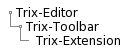
\includegraphics[scale=1]{images/dom_tree.png}
\end{center}
	\caption{Zusammenhang zwischen Trix und der Erweiterung}
\end{figure}

\section{Motivation}
Der bisher integrierte Browser-UI-Control in Fabasoft Softwareprodukten hat einige Nachteile aufgewiesen, weshalb eine Ablösung durch ein alternatives Produkt in Betracht gezogen wurde. Durch eine erste Analyse hat sich herausgestellt, dass sich der Texteditor {\em{Trix}} als Ersatz eignen könnte. Allerdings ist dieser nicht barrierefrei.

\subsection{Gleichstellung von Menschen mit Behinderungen}
In der Gesellschaft und im Alltag machen Menschen mit Behinderungen oftmals mit kleineren oder größeren Benachteiligungen Bekanntschaft. Global haben 
etwa 15 Prozent der Weltbevölkerung eine Behinderung, wobei die rund eine Milliarden Kinder und Erwachsenen assistive Technologien, wie beispielsweise 
Rollstühle oder Hörgeräte, benötigen. International hat jedes Land eine eigene Definition für den Begriff, weshalb die 
WHO (World Health Organisation, vgl. \cite{who_disability_2011}) diesen nur grob beschreiben kann. Sie geht dabei immer von drei Punkten aus:

\begin{itemize}
    \item \textbf{Impairment (dt. Schädigung)} bezeichnet jede Anomalie oder jeden Verlust der anatomischen, psychischen oder physiologischen Funktionen 
    und Strukturen des menschlichen Körpers.
    \item \textbf{Disability (dt. Beeinträchtigung)} bezeichnet jeden Mangel oder jede Einschränkung der Fähigkeiten infolge einer Beeinträchtigung, 
    wodurch eine von der Gesellschaft als normal oder in diesem Bereich betrachtete Tätigkeit nicht ausgeübt werden kann.
    \item \textbf{Handicap (dt. Behinderung)} bezeichnet den Nachteil einer Person aufgrund einer Schädigung oder Beeinträchtigung. Eine Behinderung
    steht im Zusammenhang mit einem Problem mit einer Struktur oder eines Organes des Körpers.
\end{itemize}

Grundsätzlich wird eine Behinderung in Österreich als dauerhafte Auswirkung einer körperlichen, geistigen oder psychischen Beeinträchtigung oder Beeinträchtigung
der Sinnesfunktionen bezeichnet, die einen Zeitraum von sechs Monaten überschreitet und die Teilhabe in der Gesellschaft erschwert. Damit die Benachteiligung von 
Behinderten möglichst flächendeckend beseitigt werden, verfasste das Rechtsinformationssystem des Bundes (RIS) 

\begin{itemize}
    \item das Bundesgesetz über die Gleichstellung von Menschen mit Behinderungen (Bundes-Behindertengleichstellungsgesetz - BGStG, vgl. \cite{ris_bgstg_2020}) 
    zur Regelung der Diskriminierung im täglichen Leben
    \item das Behinderteneinstellungsgesetz (BEinstG, vgl. \cite{ris_beinstg_2020}) zur Regelung der Diskriminierung in der Arbeitswelt
    \item und das Bundesgesetz vom 17. Mai 1990 über die Beratung, Betreuung und besondere Hilfe für behinderte Menschen (Bundesbehindertengesetz - BBG, vgl. \cite{ris_bbg_2020}) 
    zur Regelung der Aufgaben und Befugnisse des Behindertenanwalts.
\end{itemize}

Die Fassung des BGStG besagt, dass das Ziel die Beseitigung der Diskriminierung von Menschen mit Behinderungen sei, um diese 
gleichberechtigt am Leben in der Gesellschaft teilhaben zu lassen und eine selbstbestimmte Lebensführung zu gewährleisten.
Der Diskriminierungsschutz gilt somit für diejenigen, die körperlich, geistig, psychisch behindert oder sinnesbehindert sind, 
ebenso für ihre Angehörigen. Es ist nicht erlaubt jemanden unmittelbar oder mittelbar zu diskriminieren.

\paragraph{Definition: Diskriminierung}
Wird eine Person aufgrund ihrer Behinderung in bestimmten Situationen oder gegenüber anderen anders behandelt, so liegt eine unmittelbare Diskriminierung vor.
Eine mittelbare Diskriminierung hingegen liegt genau dann vor, wenn neutrale Vorschriften, Kriterien, Verfahren oder Merkmale gestalteter Lebensbereiche 
den Anschein erwecken Menschen mit Behinderungen gegenüber anderen auf jegliche Art und Weise zu benachteiligen.

Zu diesen Benachteiligungen gehören: 
\begin{itemize}
    \item Barrieren
    \item eine weniger günstige Behandlung
    \item Diskriminierungsaufforderungen
    \item und Belästigung aufgrund einer Behinderung
\end{itemize}

\paragraph{Arten von Behinderungen}
Grundsätzlich lassen sich Behinderungen in sechs Kategorien einteilen:

\begin{itemize}
    \item \textbf{Körperliche Behinderungen} kommen am häufigsten vor und nehmen nicht selten mit dem Alter zu. Bezeichnet werden damit starke physische 
    Einschränkungen, die auf eine Dysfunktion oder Schädigung der Stütz- und Bewegungsorgane zurückgeführt werden. Die wohl häufigste Körperbehinderung ist
    die Kinderlähmung.
    \item \textbf{Geistige Behinderungen} sind fortwährende, deutlich über dem Durchschnitt liegende Einschränkungen der kognitiven Fähigkeiten und kommen am
    zweithäufigsten vor. Zu diesen kognitiven Fähigkeiten zählen die Wahrnehmung, die Aufmerksamkeit, das Denken und das Lernen ebenso wie die Erinnerung, 
    die Motivation und die Konzentration. Das Down-Syndrom ist wohl die mit Abstand bekannteste geistige Behinderung.
    \item \textbf{Sinnesbehinderungen} umfassen alle Seh- sowie Hörbehinderungen wie Fehlsichtigkeit, Blindheit, Schwerhörigkeit, 
    Gehörlosigkeit und Taubblindheit.
    \item \textbf{Sprachbehinderungen} oder anders formuliert Störungen des Redeflusses, des Spracherwerbs, des Sprechens und der Stimme bezeichnet all jene 
    Menschen, die nicht fähig sind ihre Muttersprache im entsprechenden Alter schriftlich oder mündlich zu beherrschen. Zu den bekanntesten Sprachbehinderungen 
    gehört die Stummheit.
    \item \textbf{Psychische Behinderungen} umfassen die Beeinflussung des Denkens, Fühlens und Handelns von Menschen. Das heißt widerum, dass es Abgrenzungen
    zwischen Verhalten und Erleben gibt. Eine sehr bekannte psychische Erkrankung ist ADHS (Aufmerksamkeitsdefizit-Hyperaktivitätsstörung).
\end{itemize}

\subsection{Barrierefreiheit im Web}
\subsection{Definition: Web-Zugänglichkeit}
Web-Zugänglichkeit oder im Englischen auch ``Web Accessibility'' bezeichnet, dass alle Menschen auf dem bestmöglichen Weg Zugang zu Information 
oder Dienstleistung im Internet haben. Ziel ist es, Websites und jegliche mobile Anwendungen für alle Nutzerinnen und Nutzer, vor allem auch diejenigen mit
Behinderungen, besser zugänglich und somit barrierefrei zu gestalten. In der heutigen Gesellschaft ist das Internet mit all seinen verfügbaren Leistungen 
kaum noch wegzudenken. Zahlreiche Dienstleistungen wie etwa Onlinebanking, elektronische Dienste von Instituten und Institutionen, Onlineshop 
und viele mehr gehören dazu. Gerade aus diesem Grund ist es essenziell allen Menschen denselben Zugang zum Web zu ermöglichen.

Das Web-Zugänglichkeits-Gesetz (WZG, vlg. \cite{ris_wzg_2020}) umfasst alle rechtlichen Grundlagen 
zur Erreichung dieses Ziels. Insbesondere der Bund und alle mit ihm in Zusammenhang stehende Einrichtungen sind dazu verpflichtet barrierefreie Dienstleistungen
bereitzustellen. Hierzu gibt es bestimmte Anforderungen:

\begin{itemize}
    \item Wahrnehmbarkeit
    \item Bedienbarkeit
    \item Verständlichkeit
    \item Robustheit
\end{itemize}

Des Weiteren wurde ein zeitlicher Anwendungsbereich festgelegt, in dem alle Websites und mobile Anwendungen des Bundes barrierefrei sein müssen:

\begin{itemize}
    \item Neue Websites nach dem 23. September 2018 ab dem 23. September 2019
    \item Alte Websites vor dem 23. September 2018 ab dem 23. September 2020
    \item Alle mobilen Anwendungen ab dem 23. Juni 2021
\end{itemize}

Damit diese Dienstleistungen fortlaufend zugänglich sind, müssen die oben genannten Anforderungen regelmäßig überprüft werden. Grundsätzlich hat jede
Nutzerin und jeder Nutzer das Recht dazu, sich über Mängel bei Nichteinhaltung der Barrierefreiheit zu beschweren, die dann, wenn sie berechtigt sind, beseitigt
werden müssen. 


\section{Aufgabenstellung}
Im Rahmen dieser Diplomarbeit sollte der Texteditor {\em{Trix}} so erweitert werden, dass er den Ansprüchen für die Produkte der Fa. Fabasoft gerecht wird und von jedem Menschen einfach und ohne Probleme bedient werden kann. Inbesondere sollten die Kriterien des WCAG 2.1 (Web Content Accessibility Guidelines \cite{wcag_2_1_2018}) erfüllt werden sowie eine Bedienung mit Screenreadern und vollständig mit Tastatur ermöglicht werden.

\section{Zielsetzung}
Ziel dieser Arbeit war es, den Mitarbeiten und Kunden von Fabasoft die Verwendung eines Texteditors weiterhin zu ermöglichen sowie den bis dahin verwendeten Editor abzulösen. Des Weiteren sollten mindestens dessen bisher verfügbaren Funktionalitäten bereitgestellt werden und alle Kriterien des WCAG 2.1 erfüllt sein.

\subsection{Systemarchitektur}
% Trix ohne Erweiterung - Wie verwendet? Produkt beschreiben
\begin{figure}[H]
\begin{center}
	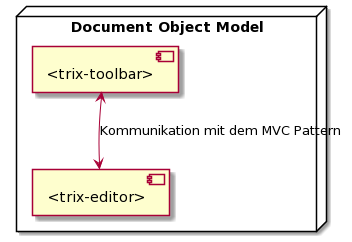
\includegraphics[scale=.6]{images/trix_components.png}
\end{center}
	\caption{Kommunikation zwischen der Toolbar und dem Editor ohne der Erweiterung}
\end{figure}

% Trix mit Erweiterung - Art von Formatvorlage, DOM Manipulation, evtl. Jenkinsfile
\begin{figure}[H]
\begin{center}
	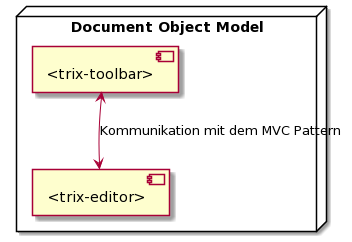
\includegraphics[scale=.6]{images/trix_components.png}
\end{center}
	\caption{Schnittstellen zwischen dem Texteditor und der Bibliothek für die Erweiterung - Durch die DOM Manipulation können zusätzlich Buttons erstellt werden, die für Trix nicht vorgesehen waren (vgl. Trix-Extension Buttons \ref{subsec:buttons})}
\end{figure}

\section{Sollzustand}
% Erweiterung genauer beschreiben

\subsection{Funktionale Anforderungen}
Die funktionalen Anforderungen an das Projekt sind:

\begin{itemize}
	\item{Aufsetzen eines Shadow-Repositories zur Erweiterung von Trix mit zusätzlichen Funktionalitäten und zur Bereitstellung der Barrierefreiheit.}
	\item{Aufsetzen eines npm-basierten Build-Prozesses mit allen notwendigen Artefakten in 
das Fabasoft npm-Repository.}
	\item{Aufbau einer Unit-Test-Infrastruktur mit einer Line-Coverage von mindestens 70 
Prozent.}
	\item{Einpflegen der entsprechenden Änderungen zur Erfüllung der Kriterien des WCAG 2.1.}
	\item{Einpflegen eines High-Level-APIs, um die Instanzierung und Parametrierung aus dem 
Fabasoft UI möglichst simpel zu gestalten.}
\end{itemize}

\subsection{Nichtfunktionale Anforderungen}

\begin{itemize}
	\item{Schlussendliche Integration in die Softwareprodukte der Fa. Fabasoft.}
	\item{Minimierung des Wartungsaufwandes.}
\end{itemize}